\chapter{系統驗證之實驗結果與討論}
\fontsize{12pt}{18pt}\selectfont %字體大小,行距

% ------------------------- 4.0 ------------------------- %
% 概述
本章節會以第三章所介紹之方法進行延伸討論,以人體的上臂肌肉為主要研究對象,藉由執行不同的動作任務,
來評估上臂特定肌肉之參數,其中以 OpenSim 與 MATLAB 軟體作為模擬與分析的工具。

% 評估對象種類;動作任務分類
本研究之上臂肌肉以肱二頭肌群為主要評估對象,其中又分為長頭與短頭兩條肌肉,代表著該肌群需要兩個希爾式肌肉模型來模擬,
而每個模型欲評估參數有三個,分別為最大等長力量 ($F^\mathrm{M}_\mathrm{O}$)、
最佳肌纖維長度 ($L^\mathrm{M}_\mathrm{O}$) 與肌腱鬆弛長度($L^\mathrm{T}_\mathrm{S}$),
動作任務則主要以手肘彎曲為主,藉由不同的彎曲方向、肩膀位置與彎曲範圍作為分類。
另外模擬案例在套用第三章方法中,不管是敏感度分析、最佳化評估還是模型驗證,用於計算之運動軌跡皆是採用關節轉動速度,
其相比於轉動角度更能呈現出細微差異,在求解的肌肉參數精準度上,也將會有更好的效果。

% ------------------------- 4.1 ------------------------- %
\section{個人化三維人體模型建立實驗結果與討論}\label{ch4_skeleton_exp}
% 實驗設定;實驗執行;結果與討論
在章節~\ref{ch3_skeleton_method} 中已詳細描述了個人化三維人體模型建立的方法,
本節使用 TotalCapture Dataset~\cite{Trumble:BMVC:2017} 提供的影片資料及相機校正數據,
嘗試建立影片中受試者的個人化三維人體模型,並進行比較及討論。

\subsection{實驗設定}
% 把 total capture dataset s1 系列做完
本章節使用 TotalCapture Dataset 之 
s1\_acting1 \textasciitilde\ s1\_acting3、s1\_freestyle1 \textasciitilde\ s1\_freestyle3、s1\_rom1 \textasciitilde\ s1\_rom3 
共九組影片資料及相機校正資料進行實驗,
每組實驗皆取用 TotalCapture Dataset 提供之相機 1 與相機 8 影像資料、兩台相機之校正資訊,
及 .bvh 檔案中 HIERARCHY 部分提供之資訊(此資訊可由 Vicon 量測而得,因此以下將稱為 Vicon 三維人體模型)。
首先,使用影像資料進行 OpenPose 影像辨識,並利用 Pose2Sim 進行相機校正及三角測量計算,建立出個人化三維人體模型,
最後取前 60 幀的資訊,計算個人化三維人體模型之平均四肢長度與 Vicon 三維人體模型之四肢長度進行比較。

\subsection{誤差評估}
% 個人化三維人體模型建立結果與驗證
% 分別評估四肢的誤差,然後再綜合再一起評估,總結誤差大概在多少內
分別計算出自行建立個人化三維人體模型的四肢長度及 Vicon 三維人體模型長度後,將兩者相減得到誤差,並計算平均誤差,
結果如表~\ref{ch3_skeleton_compare} 所示,可以發現自行建立個人化三維人體模型之四肢長度與 Vicon 三維人體模型之四肢長度相當接近,
整體平均誤差為 25.7515 (mm)。
本研究推斷,
% FIXME:推斷原因

\begin{table}[!ht]
   \caption[個人化三維人體模型建立結果與比較(mm)]{個人化三維人體模型建立結果與比較(mm)}
   \centering
   \label{ch3_skeleton_compare}
   \setlength{\tabcolsep}{3pt}
   \renewcommand\arraystretch{1.5}
   \resizebox{\textwidth}{!}{
    \begin{tabular}{c|S|S|S|S|S|S|S|S|S||S}
      & {s1\_acting1} & {s1\_acting2} & {s1\_acting3} & {s1\_freestyle1} & {s1\_freestyle2} & {s1\_freestyle3} & {s1\_rom1} & {s1\_rom2} & {s1\_rom3} & {average} \\
      \midrule[1.5pt]
      右大腿 & 15.5895 & 16.8009 & 5.8655 & 27.9576 & 24.0688 & 18.2016 & 9.7907 & 12.2067 & 1.5568 & 14.6709  \\
      右小腿 & 20.4312 & 0.7514 & 8.9552 & 11.4757 & 12.7413 & 2.5780 & 19.0733 & 20.5609 & 8.6443 & 11.6902  \\
      左大腿 & 20.1423 & 23.3496 & 14.8347 & 34.8388 & 25.4773 & 29.7342 & 18.8850 & 15.3576 & 24.7152 & 23.0372  \\
      左小腿 & 3.4795 & 7.8705 & 16.6157 & 15.0529 & 12.4442 & 15.5452 & 12.3024 & 3.2584 & 3.2571 & 9.9807  \\
      右上臂 & 37.1875 & 39.5958 & 43.2833 & 76.6637 & 59.6534 & 34.1348 & 59.4540 & 29.4289 & 32.0788 & 45.7200  \\
      右前臂 & 4.0619 & 20.9168 & 14.4801 & 59.1019 & 37.3311 & 10.6598 & 36.6949 & 4.3855 & 13.8587 & 22.3878  \\
      左上臂 & 47.6423 & 50.8824 & 51.3296 & 41.4413 & 48.9365 & 51.4196 & 36.5617 & 50.4505 & 53.2362 & 47.9889  \\
      左前臂 & 30.7583 & 24.3253 & 36.5486 & 19.8007 & 29.5842 & 34.7937 & 22.6062 & 35.9636 & 40.4441 & 30.5361  \\
      \midrule[1.5pt]
      average & 22.4116 & 23.0616 & 23.9891 & 35.7916 & 31.2796 & 24.6334 & 26.9210 & 21.4515 & 22.2239 & 25.7515  \\
   \end{tabular}}
\end{table}

\subsection{結果與討論}
% 結論
由以上誤差評估可知,本方法的整體平均誤差約為 25.75 (mm),
若僅評估人體姿勢,不延伸應用於評估手指姿勢等細微動作,則此誤差並不會造成誤判的影響,因此證明本方法確實可行。

\clearpage

% ------------------------- 4.2 ------------------------- %
\section{探討減少相機數量的可行性實驗結果與討論}
% 實驗結果
% 經過上述七類情況之實驗後,得到的 MPJPE 結果如以下所示。

\subsection{使用一台相機及八個 IMU 進行人體姿態重建實驗結果}
將圖~\ref{ch3_fig_cameraset_totalcap} 中的相機任選一台進行估計,共計有 8 種估計結果,每一結果皆可計算出 MPJPE,
MPJPE 計算結果如表~\ref{ch3_cameraset_1cam} 所示,可以發現無論選擇哪一個位置的相機,其估計誤差皆超過 500 (mm)。
標準差為 87.6016 (mm),平均值為 599.8855 (mm)。
% 因此本研究認為只使用一台相機進行估計是不可行的,至少需使用兩台相機進行量測。
\begin{table}[!ht]
   \caption[一台相機組合與其估計結果誤差]{一台相機組合與其估計結果誤差}
   \centering
   \label{ch3_cameraset_1cam}
   \setlength{\tabcolsep}{3pt}
   \renewcommand\arraystretch{1.5}
   \resizebox{\textwidth}{!}{
   \begin{tabular}{
   >{\columncolor[HTML]{E7E6E6}}c |c|
   >{\columncolor[HTML]{E7E6E6}}c |c|
   >{\columncolor[HTML]{E7E6E6}}c |c|
   >{\columncolor[HTML]{E7E6E6}}c |c}
      相機配置 & MPJPE & 相機配置 & MPJPE & 相機配置 & MPJPE & 相機配置 & MPJPE \\
      \hline
      1	& 514.76 & 2 & 782.01 & 3 & 611.84 & 4 & 520.97 \\
      5	& 653.96 & 6 & 573.41 & 7 & 599.78 & 8 & 542.36 \\
   \end{tabular}}
\end{table}
\clearpage

\subsection{使用兩台相機及八個 IMU 進行人體姿態重建實驗結果}
將圖~\ref{ch3_fig_cameraset_totalcap} 中的相機任選兩台進行排列組合,共計有 28 種組合方式之估計結果,每一結果皆可計算出 MPJPE,
MPJPE 計算結果如表~\ref{ch3_cameraset_2cam} 所示,其中最佳組合方式為相機 18,其 MPJPE 為 46.9798 (mm);
而最差組合方式為相機 25,其 MPJPE 為 300.1637 (mm)。標準差為 61.7928 (mm),平均值為 109.8694 (mm)。
經由平均值可以發現兩台相機的姿勢估計表現相對一台相機的姿勢估計表現有大幅度的進步,進步幅度約為 500 (mm);
但是由標準差可知兩台相機的姿勢估計結果仍不穩定。
% 經由結果可以發現相機的擺放位置對估計結果影響甚鉅,若位置選擇得宜,估計結果將會相當準確,反之則會有較大的誤差。
\begin{table}[!ht]
   \caption[兩台相機組合與其估計結果誤差]{兩台相機組合與其估計結果誤差}
   \centering
   \label{ch3_cameraset_2cam}
   \setlength{\tabcolsep}{3pt}
   \renewcommand\arraystretch{1.5}
   \resizebox{\textwidth}{!}{
   \begin{tabular}{
   >{\columncolor[HTML]{E7E6E6}}c |c|
   >{\columncolor[HTML]{E7E6E6}}c |c|
   >{\columncolor[HTML]{E7E6E6}}c |c|
   >{\columncolor[HTML]{E7E6E6}}c |c}
      相機配置 & MPJPE & 相機配置 & MPJPE & 相機配置 & MPJPE & 相機配置 & MPJPE \\
      \hline
      12 & 194.4957 & 13 & 81.9440 & 14 & 47.4927 & 15 & 76.7795 \\
      16 & 66.8653 & 17 & 58.7619 & 18 & 46.9798 & & \\
      \hline
      23 & 227.5722 & 24 & 182.6378 & 25 & 300.1637 & 26 & 183.0773 \\
      27 & 181.6520 & 28 & 145.2458 & & & &\\
      \hline
      34 & 99.3426 & 35 & 109.4178 & 36 & 92.7550 & 37 & 97.7435 \\
      38 & 81.3640 & & & & & &\\
      \hline
      45 & 87.4750 & 46 & 66.8800 & 47 & 67.4949 & 48 & 52.3318 \\
      \hline
      56 & 126.3387 & 57 & 95.1469 & 58 & 64.6374 & &\\
      \hline
      67 & 100.7632 & 68 & 63.7904 & & & &\\
      \hline
      78 & 77.1948 & & & & & &\\
   \end{tabular}}
\end{table}
\clearpage

\subsection{使用三台相機及八個 IMU 進行人體姿態重建實驗結果}
將圖~\ref{ch3_fig_cameraset_totalcap} 中的相機任選三台進行排列組合,共計有 56 種組合方式之估計結果,每一結果皆可計算出 MPJPE,
MPJPE 計算結果如表~\ref{ch3_cameraset_3cam} 所示,其中最佳組合方式為相機 137,其 MPJPE 為 27.1579 (mm);
而最差組合方式為相機 257,其 MPJPE 為 82.8158 (mm)。標準差為 13.8423 (mm),平均值為 42.9001 (mm)。
經由平均值可以發現:相較兩台相機的姿勢估計結果,三台相機的姿勢估計結果準確性仍有明顯提升,進步幅度約為 60 (mm);
由標準差可以知道三台相機的姿勢估計結果漸趨穩定。
% 但只要位置恰當,僅用三台相機也可以有四台相機的表現水準。
\begin{table}[!ht]
   \caption[三台相機組合與其估計結果誤差]{三台相機組合與其估計結果誤差}
   \centering
   \label{ch3_cameraset_3cam}
   \setlength{\tabcolsep}{3pt}
   \renewcommand\arraystretch{1.5}
   \resizebox{\textwidth}{!}{
   \begin{tabular}{
   >{\columncolor[HTML]{E7E6E6}}c |c|
   >{\columncolor[HTML]{E7E6E6}}c |c|
   >{\columncolor[HTML]{E7E6E6}}c |c|
   >{\columncolor[HTML]{E7E6E6}}c |c|
   >{\columncolor[HTML]{E7E6E6}}c |c}
      相機配置 & MPJPE & 相機配置 & MPJPE & 相機配置 & MPJPE & 相機配置 & MPJPE & 相機配置 & MPJPE \\
      \hline
      123 & 41.8538 & 124 & 43.2544 & 125 & 70.4747 & 126 & 41.7470 & 127 & 54.5721 \\
      128 & 46.7714 & & & & & & & & \\
      134 & 30.9862 & 135 & 29.0275 & 136 & 33.6116 & 137 & 27.1579 & 138 & 29.9961 \\
      145 & 34.4860 & 146 & 32.7227 & 147 & 29.9785 & 148 & 31.5573 & & \\
      156 & 38.3802 & 157 & 33.2107 & 158 & 33.4297 & & & & \\
      167 & 32.4098 & 168 & 33.4044 & 178 & 32.2636 & & & & \\
      \hline
      234 & 52.0193 & 235 & 76.4435 & 236 & 52.6657 & 237 & 65.5297 & 238 & 44.5936 \\
      245 & 76.6047 & 246 & 42.4841 & 247 & 54.8719 & 248 & 45.2496 & & \\
      256 & 74.8608 & 257 & 82.8158 & 258 & 62.4336 & & & & \\
      267 & 58.7578 & 268 & 39.2619 & 278 & 62.7102 & & & & \\
      \hline
      345 & 35.9928 & 346 & 42.7418 & 347 & 35.2381 & 348 & 33.5695 & & \\
      356 & 42.9933 & 357 & 35.1894 & 358 & 29.6995 & & & & \\
      367 & 40.0411 & 368 & 35.8360 & 378 & 34.9221 & & & & \\
      \hline
      456 & 40.0658 & 457 & 37.2030 & 458 & 32.7289 & & & & \\
      467 & 35.6906 & 468 & 33.8860 & 478 & 35.3151 & & & & \\
      \hline
      567 & 41.5287 & 568 & 34.8289 & 578 & 37.5083 & & & & \\
      \hline
      678 & 34.8273 & & & & & & & & \\
   \end{tabular}}
\end{table}
\clearpage

\subsection{使用四台相機及八個 IMU 進行人體姿態重建實驗結果}
將圖~\ref{ch3_fig_cameraset_totalcap} 中的相機任選四台進行排列組合,共計有 70 種組合方式之估計結果,每一結果皆可計算出 MPJPE,
MPJPE 計算結果如表~\ref{ch3_cameraset_4cam} 所示,其中最佳組合方式為相機 1357,其 MPJPE 為 24.5789 (mm);
而最差組合方式為相機 2567,其 MPJPE 為 38.9142 (mm)。標準差為 3.6860 (mm),平均值為 31.0114 (mm)。
經由平均值可以發現,四台相機的姿勢估計結果相對三台相機的姿勢估計結果有進一步提升,進步幅度約為 10 (mm),
相較兩台相機與三台相機的進步幅度有逐漸平穩的趨勢;
而由標準差可以知道四台相機組合的表現都相當穩定,無論如何選擇都不會有太大的影響。
\begin{table}[!ht]
   \caption[四台相機組合與其估計結果誤差]{四台相機組合與其估計結果誤差}
   \centering
   \label{ch3_cameraset_4cam}
   \setlength{\tabcolsep}{3pt}
   \renewcommand\arraystretch{1.5}
   \resizebox{\textwidth}{!}{
   \begin{tabular}{
   >{\columncolor[HTML]{E7E6E6}}c |c|
   >{\columncolor[HTML]{E7E6E6}}c |c|
   >{\columncolor[HTML]{E7E6E6}}c |c|
   >{\columncolor[HTML]{E7E6E6}}c |c|
   >{\columncolor[HTML]{E7E6E6}}c |c}
      % \hline
      相機配置 & MPJPE & 相機配置 & MPJPE & 相機配置 & MPJPE & 相機配置 & MPJPE & 相機配置 & MPJPE \\
      \hline
      1234 & 30.9409 & 1235 & 28.8549 & 1236 & 30.3748 & 1237 & 28.8213 & 1238 & 31.1560 \\
      1245 & 33.1706 & 1246 & 31.5377 & 1247 & 32.1031 & 1248 & 33.6613 &            &         \\
      1256 & 34.5089 & 1257 & 34.6787 & 1258 & 35.2625 &            &         &            &         \\
      1267 & 31.7009 & 1268 & 33.0636 & 1278 & 34.6861 &            &         &            &         \\
      1345 & 26.9753 & 1346 & 28.2925 & 1347 & 25.4715 & 1348 & 26.7584 &            &         \\
      1356 & 27.7651 & 1357 & 24.5789 & 1358 & 25.8578 &            &         &            &         \\
      1367 & 26.3845 & 1368 & 26.9445 & 1378 & 26.1466 &            &         &            &         \\
      1456 & 29.9311 & 1457 & 26.6848 & 1458 & 27.9429 &            &         &            &         \\
      1467 & 26.8121 & 1468 & 27.5472 & 1478 & 27.1979 &            &         &            &         \\
      1567 & 27.5824 & 1568 & 29.1892 & 1578 & 27.4552 & 1678 & 27.8378 &            &         \\
      \hline
      2345 & 34.0972 & 2346 & 36.5508 & 2347 & 36.7314 & 2348 & 33.7047 &            &         \\
      2356 & 35.6585 & 2357 & 36.3698 & 2358 & 30.8585 &            &         &            &         \\
      2367 & 36.8662 & 2368 & 32.6160 & 2378 & 34.8430 &            &         &            &         \\
      2456 & 35.6440 & 2457 & 37.1359 & 2458 & 33.4067 &            &         &            &         \\
      2467 & 35.8266 & 2468 & 33.2654 & 2478 & 36.6081 &            &         &            &         \\
      2567 & 38.9142 & 2568 & 33.7187 & 2578 & 38.7211 & 2678 & 34.3506 &            &         \\
      \hline
      3456 & 32.4429 & 3457 & 27.7338 & 3458 & 27.6554 &            &         &            &         \\
      3467 & 31.0735 & 3468 & 29.9925 & 3478 & 27.9168 &            &         &            &         \\
      3567 & 29.2876 & 3568 & 28.3170 & 3578 & 26.8460 & 3678 & 29.4004 &            &         \\
      \hline
      4567 & 29.8717 & 4568 & 29.7963 & 4578 & 28.2055 & 4678 & 28.9104 & 5678 & 29.5824 \\
   \end{tabular}}
\end{table}
\clearpage

\subsection{使用五台相機及八個 IMU 進行人體姿態重建實驗結果}
將圖~\ref{ch3_fig_cameraset_totalcap} 中的相機任選三台進行排列組合,共計有 56 種組合方式之估計結果,每一結果皆可計算出 MPJPE,
MPJPE 計算結果如表~\ref{ch3_cameraset_5cam} 所示,其中最佳組合方式為相機 13578,其 MPJPE 為 23.9568 (mm);
而最差組合方式為相機 23467,其 MPJPE 為 32.1120 (mm)。標準差為 2.0034 (mm),平均值為 27.6608 (mm)。
經由平均值可以發現:相較四台相機的姿勢估計結果,五台相機的姿勢估計結果並無明顯提升,進步幅度約為 4 (mm);
由標準差可以知道五台相機的姿勢估計結果十分集中,且將平均值與四台相機的平均值相比並無明顯進步。
\begin{table}[!ht]
   \caption[五台相機組合與其估計結果誤差]{五台相機組合與其估計結果誤差}
   \centering
   \label{ch3_cameraset_5cam}
   \setlength{\tabcolsep}{3pt}
   \renewcommand\arraystretch{1.5}
   \resizebox{\textwidth}{!}{
   \begin{tabular}{
   >{\columncolor[HTML]{E7E6E6}}c |c|
   >{\columncolor[HTML]{E7E6E6}}c |c|
   >{\columncolor[HTML]{E7E6E6}}c |c|
   >{\columncolor[HTML]{E7E6E6}}c |c|
   >{\columncolor[HTML]{E7E6E6}}c |c}
      相機配置 & MPJPE & 相機配置 & MPJPE & 相機配置 & MPJPE & 相機配置 & MPJPE & 相機配置 & MPJPE \\
      \hline
      12345 & 27.2222 & 12346 & 28.7270 & 12347 & 27.2410 & 12348 & 28.1424 & 12356 & 27.5630  \\
      12357 & 25.4345 & 12358 & 26.9508 & 12367 & 27.4309 & 12368 & 27.9631 & 12378 & 27.5871  \\
      12456 & 29.2157 & 12457 & 27.4585 & 12458 & 29.1856 & 12467 & 28.0690 & 12468 & 28.8999  \\
      12478 & 28.9294 & 12567 & 28.2794 & 12568 & 29.9585 & 12578 & 29.0917 & 12678 & 29.1141  \\
      13456 & 26.5308 & 13457 & 24.2506 & 13458 & 24.7973 & 13467 & 25.4456 & 13468 & 25.5140  \\
      13478 & 24.5152 & 13567 & 24.7163 & 13568 & 25.2622 & 13578 & 23.9568 & 13678 & 25.0847  \\
      14567 & 25.6222 & 14568 & 26.3839 & 14578 & 25.2386 & 14678 & 25.3628 & 15678 & 26.0199  \\
      \hline
      23456 & 31.3515 & 23457 & 28.8724 & 23458 & 28.4882 & 23467 & 32.1120 & 23468 & 30.4884  \\
      23478 & 29.8341 & 23567 & 29.8954 & 23568 & 28.7786 & 23578 & 27.9967 & 23678 & 30.1241  \\
      24567 & 30.4360 & 24568 & 30.1827 & 24578 & 29.4012 & 24678 & 30.1792 & 25678 & 30.1283  \\
      \hline
      34567 & 27.4939 & 34568 & 27.0215 & 34578 & 25.1997 & 34678 & 27.0385 & 35678 & 26.0327  \\
      \hline
      45678 & 26.7827 & ~ & ~ & ~ & ~ & ~ & ~ & ~ &   \\
   \end{tabular}}
\end{table}
\clearpage

\subsection{使用六台相機、七台相機與八個 IMU 進行人體姿態重建實驗結果}
由於六台相機與七台相機之估計結果皆與四台相機及五台相機的估計結果相近,因此不再完整將結果列出。
六台相機姿勢估計誤差之標準差為 1.3281 (mm),平均值為 25.9980 (mm),
七台相機姿勢估計誤差之標準差為 0.8525 (mm),平均值為 24.9272 (mm)。
將兩者的標準差及平均值與五台相機的標準差及平均值進行比較,
可以發現六台相機及七台相機的表現皆與五台相機的表現結果相近,無大幅度的進步,
因此推測增加相機數量以改善姿勢估計誤差的策略存在極限,使用四台相機即可,
再繼續增加相機數量無法顯著改善估計準確性。

\subsection{結果與討論}
% 結果介紹與討論
將一台相機到七台相機的全部 MPJPE 繪製成圖~\ref{ch3_fig_1to7cam},
可以發現相機數量從一台增加到四台時,MPJPE 隨著相機數量的增加有明顯下降的趨勢,從四台相機開始,MPJPE 的下降幅度逐漸減緩,
因此可以推斷,當相機數量增加到四台時,MPJPE 的表現已經相當穩定,且相機數量增加到五台以上時,MPJPE 的表現並不會有太大的改善。
另外,若觀察每一相機數量的最佳表現 (即 MPJPE 最小值),可以發現兩台相機及三台相機的最佳表現皆有到達誤差 50 (mm) 以下,
所以,若希望盡可能減少相機數量,且容許誤差 50 (mm),則可以選擇兩台相機或三台相機進行姿勢估計,
因此,綜上所述可推斷,為增加實驗架設方便性,減少相機數量是可考慮的選擇。
% 所以,若要達到最佳的姿勢估計結果,相機數量應選擇四台即可。
% MPJPE 約都在 20\textasciitilde40 mm 左右,只是如果三台相機的配置適當的話,結果並不會比四台相機的結果差。
\begin{figure}[!ht]
   \centering
   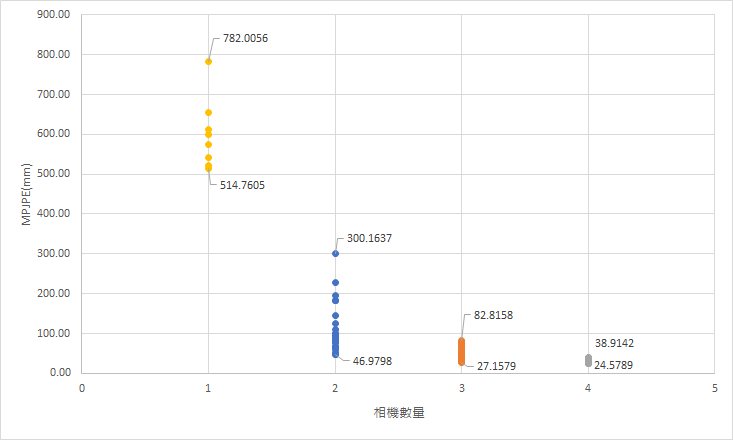
\includegraphics[width=\linewidth]{figure/ch3_fig_1to7cam.png}
   \caption[一台相機到七台相機的組合估計結果]{一台相機到七台相機的組合估計結果}
   \label{ch3_fig_1to7cam}
\end{figure}

% 跟位置討論有關的事情都先不放
% 另外列出每一相機數量的最佳表現及最差表現,如表~\ref{ch3_best_worst_camset},可以發現相機 1 皆有出現在最佳表現的結果中,而相機 2 皆有出現在最差表現的結果中,
% 因此推論相機 1 的位置較為適當。
% \begin{table}[!ht]
%    \caption[相機組合的最差及最佳表現]{相機組合的最差及最佳表現}
%    \centering
%    \label{ch3_best_worst_camset}
%    \setlength{\tabcolsep}{3pt}
%    \renewcommand\arraystretch{1.5}
%    \begin{tabular}{c|c|c|c|c}
%        & 1 cam & 2 cam & 3 cam & 4 cam \\ 
%       \midrule[2pt]
%       最差表現 & 2 & 25 & 257 & 2567 \\
%       最佳表現 & 1 & 18 & 137 & 1357 \\
%    \end{tabular}
% \end{table}

% \subsection{延伸討論}
% % 延伸討論,因為現在沒有一個比較好可以呈現這個結論的方式,所以先不放
% 由於目前文獻~\cite{Zhang_2020_CVPR}取用四台相機,因此若欲減少相機使用數量勢必會往三台相機及兩台相機的配置進行考量,
% 因此以下將進一步比較三台相機及兩台相機的估計結果,並進行討論。

% \subsubsection{方法}
% 將三台相機的估計結果依照兩台相機的配對進行平均,再與兩台相機的結果相減,以此方式觀察多一台相機的影響。
% 計算方式如算式~\ref{ch3_3camaveMin2cam}。
% \begin{equation}
%    \label{ch3_3camaveMin2cam}
%    \text{差值} = \text{ave}(\text{MPJPE}_{3 \text{ cam}})-\text{MPJPE}_{2 \text{ cam}}
% \end{equation}

% \subsubsection{結果}
% 以下表~\ref{ch3_ave_3cam_vs_2cam} 交互相機 18 為例,即將 128、138、148、158、168、178 六組相機配對的估計結果進行平均,
% 得 MPJPE = 34.5704,再與直接用兩台相機進行融合估計得到的 MPJPE = 46.9798 相減,得 12.4094。
% 由下表~\ref{ch3_ave_3cam_vs_2cam} 可知,相機 1 及相機 8 的配對再加上第三台相機較不會有顯著的改善,
% 且前三種配對 (即配對 18、配對 14、配對 48)的改善皆都落在約 10~15 mm 左右,
% 所以可以推斷,相機 1、4、8 三個位置,隨意取其中兩者可能是較適合擺放相機的位置。
% \begin{table}[!ht]
%    \caption[兩台相機與三台相機平均之比較]{兩台相機與三台相機平均之比較}
%    \centering
%    \label{ch3_ave_3cam_vs_2cam}
%    \setlength{\tabcolsep}{3pt}
%    \renewcommand\arraystretch{1.5}
%    \begin{tabular}{c|c|c|c}
%       交互相機 & $ave(MPJPE_{3 cam})$ & $MPJPE_{2 cam}$ & 差 \\
%       \midrule[2pt]
%       18 & 34.5704 & 46.9798 & 12.4094 \\
%       14 & 33.8308 & 47.4927 & 13.6619 \\
%       48 & 35.3844 & 52.3318 & 16.9474 \\
%       17 & 34.9321 & 58.7619 & 23.8298 \\ 
%       58 & 38.4382 & 64.6374 & 26.1993 \\
%       68 & 35.3408 & 63.7904 & 28.4496 \\
%       46 & 37.9318 & 66.8800 & 28.9481 \\  
%       47 & 38.0495 & 67.4949 & 29.4454 \\ 
%       16 & 35.3793 & 66.8653 & 31.4860 \\ 
%       15 & 39.8348 & 76.7795 & 36.9447 \\
%       78 & 39.5911 & 77.1948 & 37.6037 \\
%    \end{tabular}
% \end{table}

% 另外,若希望 $MPJPE_{2 cam}$ 低於 80 mm,則從兩台相機的估計結果(表~\ref{ch3_cameraset_2cam})挑選出 $MPJPE_{2 cam}$ 低於 80 mm 的結果,
% 並計算每一相機的出現次數,則可得出如下表~\ref{ch3_cam_occurrence} 的結果,觀察下表也可發現相機 1、8 的出現次數最高,
% 其次為相機 4 ,因此也可推斷相機 1、4、8 三個位置可能是較適合擺放相機的位置。
% \begin{table}[!ht]
%    \caption[兩台相機估計結果之每台相機的出現次數]{兩台相機估計結果之每台相機的出現次數}
%    \centering
%    \label{ch3_cam_occurrence}
%    \setlength{\tabcolsep}{3pt}
%    \renewcommand\arraystretch{1.5}
%    \begin{tabular}{c|c}
%       相機 & 出現次數 \\
%       \midrule[2pt]
%       1 & 5 \\
%       2 & 0 \\
%       3 & 0 \\
%       4 & 4 \\
%       5 & 2 \\
%       6 & 3 \\
%       7 & 3 \\
%       8 & 5 \\
%    \end{tabular}
% \end{table}

% ------------------------- 4.3 ------------------------- %
\section{使用影像辨識於室內估計姿態}
單獨 heatmap 的結果
\subsection{實驗設定}
% 實驗設定
123123
% \subsection{實驗執行}
% % 實驗執行
% 123123
\subsection{誤差評估}
% 誤差評估
123123
\subsection{結論}
% 結論
123123

% % ------------------------- 4.3 ------------------------- %
% \section{單獨做 IMU 的姿勢估計}
% 單獨 IMU 的結果
% \subsection{實驗設定}
% % 實驗設定
% 123123
% \subsection{實驗執行}
% % 實驗執行
% 123123
% \subsection{誤差評估}
% % 誤差評估
% 123123
% \subsection{結論}
% % 結論
% 123123

% ------------------------- 4.4 ------------------------- %
\section{使用影像辨識融合 IMU 於室內估計姿態}
sensor fusion 在室內的結果
\subsection{實驗設定}
% 實驗設定
123123
% \subsection{實驗執行}
% % 實驗執行
% 123123
\subsection{誤差評估}
% 誤差評估
123123
\subsection{結論}
% 結論
123123

% ------------------------- 4.5 ------------------------- %
\section{使用影像辨識融合 IMU 於室外估計姿態}
sensor fusion 在室外的結果
\subsection{實驗設定}
% 實驗設定
123123
% \subsection{實驗執行}
% % 實驗執行
% 123123
\subsection{誤差評估}
% 誤差評估
123123
\subsection{結論}
% 結論
123123

% ------------------------- 4.6 ------------------------- %
\section{小結}
% 回顧;下章節再討論;從驗證結果證實方法有效
本章節將上肢肌肉骨骼模型套用在所提出的研究方法,介紹了許多模擬案例的細節,如負重功能的新增、運動軌跡公式、
任務種類等資訊,除此之外也先透過該模型來展示敏感度分析的結果,提供後續的最佳化與模型驗證的任務挑選,
最主要的目的是要完成上肢特定肌肉之參數評估。下個章節將依據第三章的研究方法、第四章的前置作業,
完整介紹參數評估案例,並針對評估結果進行探討。

\clearpage